\documentclass[12pt,]{article}
\usepackage{lmodern}
\usepackage{amssymb,amsmath}
\usepackage{ifxetex,ifluatex}
\usepackage{fixltx2e} % provides \textsubscript
\ifnum 0\ifxetex 1\fi\ifluatex 1\fi=0 % if pdftex
  \usepackage[T1]{fontenc}
  \usepackage[utf8]{inputenc}
\else % if luatex or xelatex
  \ifxetex
    \usepackage{mathspec}
  \else
    \usepackage{fontspec}
  \fi
  \defaultfontfeatures{Ligatures=TeX,Scale=MatchLowercase}
\fi
% use upquote if available, for straight quotes in verbatim environments
\IfFileExists{upquote.sty}{\usepackage{upquote}}{}
% use microtype if available
\IfFileExists{microtype.sty}{%
\usepackage{microtype}
\UseMicrotypeSet[protrusion]{basicmath} % disable protrusion for tt fonts
}{}
\usepackage[margin=1in]{geometry}
\usepackage{hyperref}
\hypersetup{unicode=true,
            pdftitle={Report about E-colored Diamonds},
            pdfauthor={Hanna Tillmanns (WIdO)},
            pdfborder={0 0 0},
            breaklinks=true}
\urlstyle{same}  % don't use monospace font for urls
\usepackage{color}
\usepackage{fancyvrb}
\newcommand{\VerbBar}{|}
\newcommand{\VERB}{\Verb[commandchars=\\\{\}]}
\DefineVerbatimEnvironment{Highlighting}{Verbatim}{commandchars=\\\{\}}
% Add ',fontsize=\small' for more characters per line
\usepackage{framed}
\definecolor{shadecolor}{RGB}{248,248,248}
\newenvironment{Shaded}{\begin{snugshade}}{\end{snugshade}}
\newcommand{\KeywordTok}[1]{\textcolor[rgb]{0.13,0.29,0.53}{\textbf{#1}}}
\newcommand{\DataTypeTok}[1]{\textcolor[rgb]{0.13,0.29,0.53}{#1}}
\newcommand{\DecValTok}[1]{\textcolor[rgb]{0.00,0.00,0.81}{#1}}
\newcommand{\BaseNTok}[1]{\textcolor[rgb]{0.00,0.00,0.81}{#1}}
\newcommand{\FloatTok}[1]{\textcolor[rgb]{0.00,0.00,0.81}{#1}}
\newcommand{\ConstantTok}[1]{\textcolor[rgb]{0.00,0.00,0.00}{#1}}
\newcommand{\CharTok}[1]{\textcolor[rgb]{0.31,0.60,0.02}{#1}}
\newcommand{\SpecialCharTok}[1]{\textcolor[rgb]{0.00,0.00,0.00}{#1}}
\newcommand{\StringTok}[1]{\textcolor[rgb]{0.31,0.60,0.02}{#1}}
\newcommand{\VerbatimStringTok}[1]{\textcolor[rgb]{0.31,0.60,0.02}{#1}}
\newcommand{\SpecialStringTok}[1]{\textcolor[rgb]{0.31,0.60,0.02}{#1}}
\newcommand{\ImportTok}[1]{#1}
\newcommand{\CommentTok}[1]{\textcolor[rgb]{0.56,0.35,0.01}{\textit{#1}}}
\newcommand{\DocumentationTok}[1]{\textcolor[rgb]{0.56,0.35,0.01}{\textbf{\textit{#1}}}}
\newcommand{\AnnotationTok}[1]{\textcolor[rgb]{0.56,0.35,0.01}{\textbf{\textit{#1}}}}
\newcommand{\CommentVarTok}[1]{\textcolor[rgb]{0.56,0.35,0.01}{\textbf{\textit{#1}}}}
\newcommand{\OtherTok}[1]{\textcolor[rgb]{0.56,0.35,0.01}{#1}}
\newcommand{\FunctionTok}[1]{\textcolor[rgb]{0.00,0.00,0.00}{#1}}
\newcommand{\VariableTok}[1]{\textcolor[rgb]{0.00,0.00,0.00}{#1}}
\newcommand{\ControlFlowTok}[1]{\textcolor[rgb]{0.13,0.29,0.53}{\textbf{#1}}}
\newcommand{\OperatorTok}[1]{\textcolor[rgb]{0.81,0.36,0.00}{\textbf{#1}}}
\newcommand{\BuiltInTok}[1]{#1}
\newcommand{\ExtensionTok}[1]{#1}
\newcommand{\PreprocessorTok}[1]{\textcolor[rgb]{0.56,0.35,0.01}{\textit{#1}}}
\newcommand{\AttributeTok}[1]{\textcolor[rgb]{0.77,0.63,0.00}{#1}}
\newcommand{\RegionMarkerTok}[1]{#1}
\newcommand{\InformationTok}[1]{\textcolor[rgb]{0.56,0.35,0.01}{\textbf{\textit{#1}}}}
\newcommand{\WarningTok}[1]{\textcolor[rgb]{0.56,0.35,0.01}{\textbf{\textit{#1}}}}
\newcommand{\AlertTok}[1]{\textcolor[rgb]{0.94,0.16,0.16}{#1}}
\newcommand{\ErrorTok}[1]{\textcolor[rgb]{0.64,0.00,0.00}{\textbf{#1}}}
\newcommand{\NormalTok}[1]{#1}
\usepackage{longtable,booktabs}
\usepackage{graphicx,grffile}
\makeatletter
\def\maxwidth{\ifdim\Gin@nat@width>\linewidth\linewidth\else\Gin@nat@width\fi}
\def\maxheight{\ifdim\Gin@nat@height>\textheight\textheight\else\Gin@nat@height\fi}
\makeatother
% Scale images if necessary, so that they will not overflow the page
% margins by default, and it is still possible to overwrite the defaults
% using explicit options in \includegraphics[width, height, ...]{}
\setkeys{Gin}{width=\maxwidth,height=\maxheight,keepaspectratio}
\IfFileExists{parskip.sty}{%
\usepackage{parskip}
}{% else
\setlength{\parindent}{0pt}
\setlength{\parskip}{6pt plus 2pt minus 1pt}
}
\setlength{\emergencystretch}{3em}  % prevent overfull lines
\providecommand{\tightlist}{%
  \setlength{\itemsep}{0pt}\setlength{\parskip}{0pt}}
\setcounter{secnumdepth}{5}

%%% Use protect on footnotes to avoid problems with footnotes in titles
\let\rmarkdownfootnote\footnote%
\def\footnote{\protect\rmarkdownfootnote}

%%% Change title format to be more compact
\usepackage{titling}

% Create subtitle command for use in maketitle
\providecommand{\subtitle}[1]{
  \posttitle{
    \begin{center}\large#1\end{center}
    }
}

\setlength{\droptitle}{-2em}

  \title{\vspace{3in}Report about E-colored Diamonds}
    \pretitle{\vspace{\droptitle}\centering\huge}
  \posttitle{\par}
    \author{Hanna Tillmanns (WIdO)}
    \preauthor{\centering\large\emph}
  \postauthor{\par}
      \predate{\centering\large\emph}
  \postdate{\par}
    \date{Stand: 14.06.2019}

\renewcommand{\contentsname}{}

\begin{document}
\maketitle

{
\setcounter{tocdepth}{2}
\tableofcontents
}
\section{\texorpdfstring{Defining parameters ``outside'' the
script}{Defining parameters outside the script}}\label{defining-parameters-outside-the-script}

To be able to render the scripts with different parameters and not
having to start it by hand, I use the ``params''-value of the YAML.

The scripts are then startet with rmarkdown::render.

\section{Define all the general things and import the
data}\label{define-all-the-general-things-and-import-the-data}

First things first. At the beginning I load all libraries, define the
general parameters and import all of the data. In my case importing the
data takes some time, therefore it is nice not having to repeat this for
every single child-script, especially those that run several times.

\begin{Shaded}
\begin{Highlighting}[]
\CommentTok{# define parames}
\NormalTok{col<-}\StringTok{ }\NormalTok{params}\OperatorTok{$}\NormalTok{col}


\CommentTok{#load librarys}

\KeywordTok{library}\NormalTok{(openxlsx)}
\CommentTok{#library(reshape2)}
\CommentTok{#library (RODBC)}
\CommentTok{#library(lmtest)}
\CommentTok{#library(ggplot2)}
\KeywordTok{library}\NormalTok{(foreach)}
\KeywordTok{library}\NormalTok{(tidyverse)           }
\CommentTok{#library(treemap)}
\CommentTok{#library(gridExtra)  }
\CommentTok{#library(grid)      }
\KeywordTok{library}\NormalTok{(knitr) }
\CommentTok{#library(pander)}
\CommentTok{#library(kableExtra) }
\CommentTok{#library(captioner) }
\CommentTok{#library(here)}
\CommentTok{#library(RGraphics)}
\CommentTok{#library(treemapify)}


\CommentTok{#Creating the Data for the Report}

\NormalTok{data <-}\StringTok{ }\NormalTok{diamonds }\OperatorTok\StringTok{ }
\StringTok{  }\KeywordTok{filter}\NormalTok{(color}\OperatorTok{==}\NormalTok{col)}
\end{Highlighting}
\end{Shaded}

\section{Creating the Report}\label{creating-the-report}

The report can be divided into different types of sections:

\begin{itemize}
\tightlist
\item
  all those sections that are within the parent script
\item
  sections that are in child-scripts
\item
  without a loop and without a condition
\item
  with a condition that has to be true to render the file
\item
  within a loop, which creates a section for every defined specificaton.
\end{itemize}

\section{Single child-script}\label{single-child-script}

\begin{Shaded}
\begin{Highlighting}[]
\CommentTok{# calling a single child with}

\CommentTok{#```\{r single_child,child = 'Single_Child.rmd'\}}
\CommentTok{#```}
\end{Highlighting}
\end{Shaded}

\subsection{Start Child-Script}\label{start-child-script}

The section gets all the parameters and data from the parent script.

Myselfe use it mainly for organising my script.

\begin{Shaded}
\begin{Highlighting}[]
  \KeywordTok{ggplot}\NormalTok{(}\DataTypeTok{data=}\NormalTok{data) }\OperatorTok{+}\StringTok{ }
\StringTok{  }\KeywordTok{geom_bar}\NormalTok{(}\KeywordTok{aes}\NormalTok{(}\DataTypeTok{x=}\NormalTok{cut)) }\OperatorTok{+}
\StringTok{  }\KeywordTok{labs}\NormalTok{(}\DataTypeTok{title=}\KeywordTok{paste0}\NormalTok{(}\StringTok{"Diamonds of the color "}\NormalTok{,col))}
\end{Highlighting}
\end{Shaded}

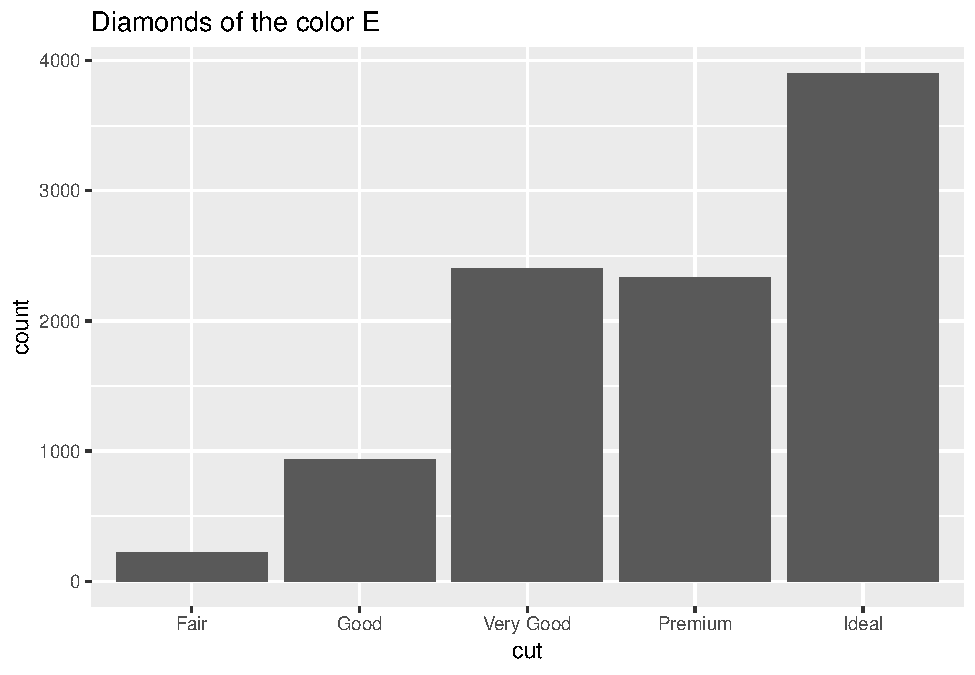
\includegraphics{SatRDay_Example_automatedReports_files/figure-latex/unnamed-chunk-3-1.pdf}

\section{Conditional child-script}\label{conditional-child-script}

The script will only be evaluated if the condition is true. This is a
nice way to cope for example with missing data.

\begin{Shaded}
\begin{Highlighting}[]
\CommentTok{#creating the test}

\NormalTok{test <-}\StringTok{ }\KeywordTok{ifelse}\NormalTok{(data }\OperatorTok\StringTok{ }
\StringTok{                   }\KeywordTok{filter}\NormalTok{(clarity}\OperatorTok{==}\StringTok{"SI2"}\NormalTok{) }\OperatorTok\StringTok{ }\KeywordTok{nrow}\NormalTok{()}\OperatorTok{>}\DecValTok{0}\NormalTok{,}\OtherTok{TRUE}\NormalTok{,}\OtherTok{FALSE}\NormalTok{)}
\end{Highlighting}
\end{Shaded}

\begin{Shaded}
\begin{Highlighting}[]
\CommentTok{#calling the conditional child-script with: }

\CommentTok{#```\{r conditional_print_script, child='cond_child.Rmd', eval = test\}}
\CommentTok{#```}
\end{Highlighting}
\end{Shaded}

\subsection{Start conditional
child-script}\label{start-conditional-child-script}

The average price of diamonds with the clarity ``SI2'' is 4173.8260362.

\section{Looping over child-scripts}\label{looping-over-child-scripts}

As the names of chunks may not be repeated, the chunks should be
nameless.

\begin{Shaded}
\begin{Highlighting}[]
\NormalTok{  out.loop<-}\OtherTok{NULL} \CommentTok{#creating the output}
  
\CommentTok{#Creating a chapter for every cut}

\KeywordTok{foreach}\NormalTok{(}\DataTypeTok{y=} \KeywordTok{c}\NormalTok{(}\StringTok{"Premium"}\NormalTok{,}\StringTok{"Fair"}\NormalTok{)) }\OperatorTok\StringTok{ }\NormalTok{\{  }
  
  \CommentTok{#Parameters used within the loop can be created}
  
\NormalTok{  cut.short <-}\StringTok{ }\KeywordTok{case_when}\NormalTok{(y}\OperatorTok{==}\StringTok{"Ideal"}\OperatorTok{~}\StringTok{"I"}\NormalTok{,}
\NormalTok{                         y}\OperatorTok{==}\StringTok{"Premium"}\OperatorTok{~}\StringTok{"P"}\NormalTok{,}
\NormalTok{                         y}\OperatorTok{==}\StringTok{"Good"}\OperatorTok{~}\StringTok{"G"}\NormalTok{,}
\NormalTok{                         y}\OperatorTok{==}\StringTok{"Very Good"}\OperatorTok{~}\StringTok{"V"}\NormalTok{,}
\NormalTok{                         y}\OperatorTok{==}\StringTok{"Fair"}\OperatorTok{~}\StringTok{"F"}
\NormalTok{                         )}
\NormalTok{  headline<-}\StringTok{  }\KeywordTok{paste0}\NormalTok{(}\StringTok{"# Section about the cut "}\NormalTok{, y)}
  
  \CommentTok{#Creating the chapter for every cut}
  
\NormalTok{  res.loop<-}\KeywordTok{c}\NormalTok{(headline  }
\NormalTok{      ,   }\KeywordTok{knit_child}\NormalTok{(}\StringTok{'loop_child_1.Rmd'}\NormalTok{ , }\DataTypeTok{envir=}\KeywordTok{knit_global}\NormalTok{())  }
\NormalTok{      ,   }\KeywordTok{knit_child}\NormalTok{(}\StringTok{'loop_child_2.RMD'}\NormalTok{ , }\DataTypeTok{envir=}\KeywordTok{knit_global}\NormalTok{())       }
\NormalTok{                      )}
  
  \CommentTok{#Puting the chapters together}
  
\NormalTok{  out.loop <-}\StringTok{ }\KeywordTok{c}\NormalTok{(out.loop,res.loop)}
  
\NormalTok{  \}}
\end{Highlighting}
\end{Shaded}

\newpage

\begin{Shaded}
\begin{Highlighting}[]
\CommentTok{#Pasting the chapters into the text with the following inline code}

\CommentTok{# `r  paste(out.loop, collapse='\textbackslash{}n')`}
\end{Highlighting}
\end{Shaded}

\section{Section about the cut
Premium}\label{section-about-the-cut-premium}

\subsection{First child-script}\label{first-child-script}

\begin{Shaded}
\begin{Highlighting}[]
\NormalTok{data }\OperatorTok\StringTok{ }
\StringTok{  }\KeywordTok{filter}\NormalTok{(}\KeywordTok{substr}\NormalTok{(cut,}\DecValTok{1}\NormalTok{,}\DecValTok{1}\NormalTok{)}\OperatorTok{==}\NormalTok{cut.short) }\OperatorTok\StringTok{ }
\StringTok{  }\KeywordTok{group_by}\NormalTok{(price) }\OperatorTok\StringTok{ }
\StringTok{  }\KeywordTok{summarise}\NormalTok{(}\DataTypeTok{nu=}\KeywordTok{n}\NormalTok{()) }\OperatorTok\StringTok{ }
\StringTok{  }\KeywordTok{arrange}\NormalTok{(price) }\OperatorTok\StringTok{ }
\StringTok{  }\KeywordTok{mutate}\NormalTok{(}\DataTypeTok{per=}\KeywordTok{cumsum}\NormalTok{(nu)}\OperatorTok{/}\KeywordTok{sum}\NormalTok{(nu)}\OperatorTok{*}\DecValTok{100}\NormalTok{) }\OperatorTok\StringTok{ }
\StringTok{  }\KeywordTok{ggplot}\NormalTok{()}\OperatorTok{+}\KeywordTok{geom_line}\NormalTok{(}\KeywordTok{aes}\NormalTok{(}\DataTypeTok{x=}\NormalTok{price,}\DataTypeTok{y=}\NormalTok{per)) }\OperatorTok{+}
\StringTok{  }\KeywordTok{labs}\NormalTok{(}\DataTypeTok{title =} \KeywordTok{paste0}\NormalTok{(}\StringTok{"Overview of prices of diamonds of cut "}\NormalTok{,y),}
       \DataTypeTok{y=}\StringTok{"cumulated share"}\NormalTok{)}
\end{Highlighting}
\end{Shaded}

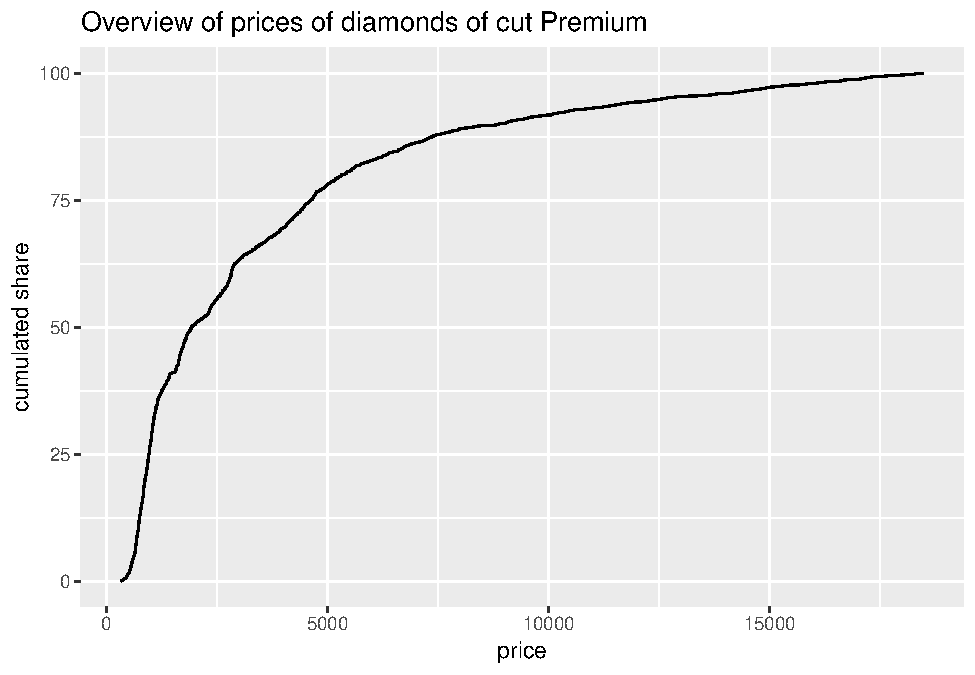
\includegraphics{SatRDay_Example_automatedReports_files/figure-latex/unnamed-chunk-4-1.pdf}

\subsection{Second child-script}\label{second-child-script}

\begin{Shaded}
\begin{Highlighting}[]
\NormalTok{t<-}
\NormalTok{data }\OperatorTok\StringTok{ }
\StringTok{  }\KeywordTok{filter}\NormalTok{(}\KeywordTok{substr}\NormalTok{(cut,}\DecValTok{1}\NormalTok{,}\DecValTok{1}\NormalTok{)}\OperatorTok{==}\NormalTok{cut.short}\OperatorTok{&}\NormalTok{price}\OperatorTok{>=}\DecValTok{16000}\NormalTok{) }\OperatorTok\StringTok{ }
\StringTok{  }\KeywordTok{summarise}\NormalTok{(}\DataTypeTok{t=}\KeywordTok{n}\NormalTok{()) }\OperatorTok\StringTok{ }\KeywordTok{pull}\NormalTok{(t)}
\end{Highlighting}
\end{Shaded}

48 Diamonds of the cut Premium have a price higher than 16.000.

\newpage

\section{Section about the cut Fair}\label{section-about-the-cut-fair}

\subsection{First child-script}\label{first-child-script-1}

\begin{Shaded}
\begin{Highlighting}[]
\NormalTok{data }\OperatorTok\StringTok{ }
\StringTok{  }\KeywordTok{filter}\NormalTok{(}\KeywordTok{substr}\NormalTok{(cut,}\DecValTok{1}\NormalTok{,}\DecValTok{1}\NormalTok{)}\OperatorTok{==}\NormalTok{cut.short) }\OperatorTok\StringTok{ }
\StringTok{  }\KeywordTok{group_by}\NormalTok{(price) }\OperatorTok\StringTok{ }
\StringTok{  }\KeywordTok{summarise}\NormalTok{(}\DataTypeTok{nu=}\KeywordTok{n}\NormalTok{()) }\OperatorTok\StringTok{ }
\StringTok{  }\KeywordTok{arrange}\NormalTok{(price) }\OperatorTok\StringTok{ }
\StringTok{  }\KeywordTok{mutate}\NormalTok{(}\DataTypeTok{per=}\KeywordTok{cumsum}\NormalTok{(nu)}\OperatorTok{/}\KeywordTok{sum}\NormalTok{(nu)}\OperatorTok{*}\DecValTok{100}\NormalTok{) }\OperatorTok\StringTok{ }
\StringTok{  }\KeywordTok{ggplot}\NormalTok{()}\OperatorTok{+}\KeywordTok{geom_line}\NormalTok{(}\KeywordTok{aes}\NormalTok{(}\DataTypeTok{x=}\NormalTok{price,}\DataTypeTok{y=}\NormalTok{per)) }\OperatorTok{+}
\StringTok{  }\KeywordTok{labs}\NormalTok{(}\DataTypeTok{title =} \KeywordTok{paste0}\NormalTok{(}\StringTok{"Overview of prices of diamonds of cut "}\NormalTok{,y),}
       \DataTypeTok{y=}\StringTok{"cumulated share"}\NormalTok{)}
\end{Highlighting}
\end{Shaded}

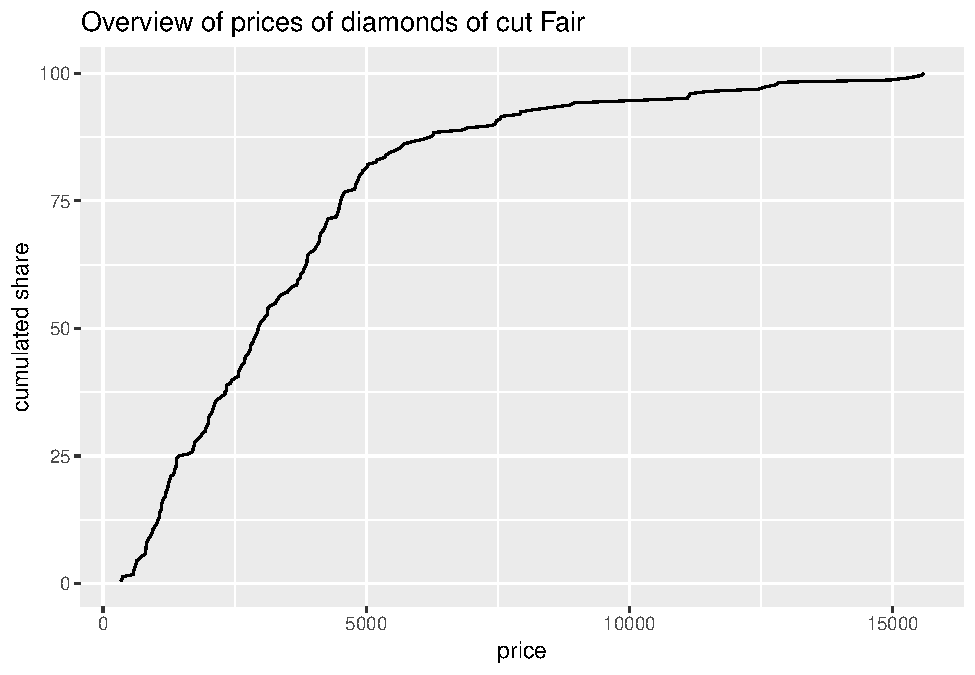
\includegraphics{SatRDay_Example_automatedReports_files/figure-latex/unnamed-chunk-6-1.pdf}

\subsection{Second child-script}\label{second-child-script-1}

\begin{Shaded}
\begin{Highlighting}[]
\NormalTok{t<-}
\NormalTok{data }\OperatorTok\StringTok{ }
\StringTok{  }\KeywordTok{filter}\NormalTok{(}\KeywordTok{substr}\NormalTok{(cut,}\DecValTok{1}\NormalTok{,}\DecValTok{1}\NormalTok{)}\OperatorTok{==}\NormalTok{cut.short}\OperatorTok{&}\NormalTok{price}\OperatorTok{>=}\DecValTok{16000}\NormalTok{) }\OperatorTok\StringTok{ }
\StringTok{  }\KeywordTok{summarise}\NormalTok{(}\DataTypeTok{t=}\KeywordTok{n}\NormalTok{()) }\OperatorTok\StringTok{ }\KeywordTok{pull}\NormalTok{(t)}
\end{Highlighting}
\end{Shaded}

0 Diamonds of the cut Fair have a price higher than 16.000.

\newpage


\end{document}
